% Options for packages loaded elsewhere
\PassOptionsToPackage{unicode}{hyperref}
\PassOptionsToPackage{hyphens}{url}
%
\documentclass[
]{article}
\usepackage{amsmath,amssymb}
\usepackage{iftex}
\ifPDFTeX
  \usepackage[T1]{fontenc}
  \usepackage[utf8]{inputenc}
  \usepackage{textcomp} % provide euro and other symbols
\else % if luatex or xetex
  \usepackage{unicode-math} % this also loads fontspec
  \defaultfontfeatures{Scale=MatchLowercase}
  \defaultfontfeatures[\rmfamily]{Ligatures=TeX,Scale=1}
\fi
\usepackage{lmodern}
\ifPDFTeX\else
  % xetex/luatex font selection
\fi
% Use upquote if available, for straight quotes in verbatim environments
\IfFileExists{upquote.sty}{\usepackage{upquote}}{}
\IfFileExists{microtype.sty}{% use microtype if available
  \usepackage[]{microtype}
  \UseMicrotypeSet[protrusion]{basicmath} % disable protrusion for tt fonts
}{}
\makeatletter
\@ifundefined{KOMAClassName}{% if non-KOMA class
  \IfFileExists{parskip.sty}{%
    \usepackage{parskip}
  }{% else
    \setlength{\parindent}{0pt}
    \setlength{\parskip}{6pt plus 2pt minus 1pt}}
}{% if KOMA class
  \KOMAoptions{parskip=half}}
\makeatother
\usepackage{xcolor}
\usepackage[margin=1in]{geometry}
\usepackage{color}
\usepackage{fancyvrb}
\newcommand{\VerbBar}{|}
\newcommand{\VERB}{\Verb[commandchars=\\\{\}]}
\DefineVerbatimEnvironment{Highlighting}{Verbatim}{commandchars=\\\{\}}
% Add ',fontsize=\small' for more characters per line
\usepackage{framed}
\definecolor{shadecolor}{RGB}{248,248,248}
\newenvironment{Shaded}{\begin{snugshade}}{\end{snugshade}}
\newcommand{\AlertTok}[1]{\textcolor[rgb]{0.94,0.16,0.16}{#1}}
\newcommand{\AnnotationTok}[1]{\textcolor[rgb]{0.56,0.35,0.01}{\textbf{\textit{#1}}}}
\newcommand{\AttributeTok}[1]{\textcolor[rgb]{0.13,0.29,0.53}{#1}}
\newcommand{\BaseNTok}[1]{\textcolor[rgb]{0.00,0.00,0.81}{#1}}
\newcommand{\BuiltInTok}[1]{#1}
\newcommand{\CharTok}[1]{\textcolor[rgb]{0.31,0.60,0.02}{#1}}
\newcommand{\CommentTok}[1]{\textcolor[rgb]{0.56,0.35,0.01}{\textit{#1}}}
\newcommand{\CommentVarTok}[1]{\textcolor[rgb]{0.56,0.35,0.01}{\textbf{\textit{#1}}}}
\newcommand{\ConstantTok}[1]{\textcolor[rgb]{0.56,0.35,0.01}{#1}}
\newcommand{\ControlFlowTok}[1]{\textcolor[rgb]{0.13,0.29,0.53}{\textbf{#1}}}
\newcommand{\DataTypeTok}[1]{\textcolor[rgb]{0.13,0.29,0.53}{#1}}
\newcommand{\DecValTok}[1]{\textcolor[rgb]{0.00,0.00,0.81}{#1}}
\newcommand{\DocumentationTok}[1]{\textcolor[rgb]{0.56,0.35,0.01}{\textbf{\textit{#1}}}}
\newcommand{\ErrorTok}[1]{\textcolor[rgb]{0.64,0.00,0.00}{\textbf{#1}}}
\newcommand{\ExtensionTok}[1]{#1}
\newcommand{\FloatTok}[1]{\textcolor[rgb]{0.00,0.00,0.81}{#1}}
\newcommand{\FunctionTok}[1]{\textcolor[rgb]{0.13,0.29,0.53}{\textbf{#1}}}
\newcommand{\ImportTok}[1]{#1}
\newcommand{\InformationTok}[1]{\textcolor[rgb]{0.56,0.35,0.01}{\textbf{\textit{#1}}}}
\newcommand{\KeywordTok}[1]{\textcolor[rgb]{0.13,0.29,0.53}{\textbf{#1}}}
\newcommand{\NormalTok}[1]{#1}
\newcommand{\OperatorTok}[1]{\textcolor[rgb]{0.81,0.36,0.00}{\textbf{#1}}}
\newcommand{\OtherTok}[1]{\textcolor[rgb]{0.56,0.35,0.01}{#1}}
\newcommand{\PreprocessorTok}[1]{\textcolor[rgb]{0.56,0.35,0.01}{\textit{#1}}}
\newcommand{\RegionMarkerTok}[1]{#1}
\newcommand{\SpecialCharTok}[1]{\textcolor[rgb]{0.81,0.36,0.00}{\textbf{#1}}}
\newcommand{\SpecialStringTok}[1]{\textcolor[rgb]{0.31,0.60,0.02}{#1}}
\newcommand{\StringTok}[1]{\textcolor[rgb]{0.31,0.60,0.02}{#1}}
\newcommand{\VariableTok}[1]{\textcolor[rgb]{0.00,0.00,0.00}{#1}}
\newcommand{\VerbatimStringTok}[1]{\textcolor[rgb]{0.31,0.60,0.02}{#1}}
\newcommand{\WarningTok}[1]{\textcolor[rgb]{0.56,0.35,0.01}{\textbf{\textit{#1}}}}
\usepackage{graphicx}
\makeatletter
\def\maxwidth{\ifdim\Gin@nat@width>\linewidth\linewidth\else\Gin@nat@width\fi}
\def\maxheight{\ifdim\Gin@nat@height>\textheight\textheight\else\Gin@nat@height\fi}
\makeatother
% Scale images if necessary, so that they will not overflow the page
% margins by default, and it is still possible to overwrite the defaults
% using explicit options in \includegraphics[width, height, ...]{}
\setkeys{Gin}{width=\maxwidth,height=\maxheight,keepaspectratio}
% Set default figure placement to htbp
\makeatletter
\def\fps@figure{htbp}
\makeatother
\setlength{\emergencystretch}{3em} % prevent overfull lines
\providecommand{\tightlist}{%
  \setlength{\itemsep}{0pt}\setlength{\parskip}{0pt}}
\setcounter{secnumdepth}{-\maxdimen} % remove section numbering
\ifLuaTeX
  \usepackage{selnolig}  % disable illegal ligatures
\fi
\IfFileExists{bookmark.sty}{\usepackage{bookmark}}{\usepackage{hyperref}}
\IfFileExists{xurl.sty}{\usepackage{xurl}}{} % add URL line breaks if available
\urlstyle{same}
\hypersetup{
  pdftitle={Sesión 3},
  hidelinks,
  pdfcreator={LaTeX via pandoc}}

\title{Sesión 3}
\author{}
\date{\vspace{-2.5em}}

\begin{document}
\maketitle

{
\setcounter{tocdepth}{1}
\tableofcontents
}
\begin{flushleft}
\includegraphics[width=0.3\linewidth]{logoPUCP} \end{flushleft}

\hypertarget{facultad-de-ciencias-sociales---pucp}{%
\subsection{\texorpdfstring{FACULTAD DE CIENCIAS SOCIALES - PUCP
}{FACULTAD DE CIENCIAS SOCIALES - PUCP  }}\label{facultad-de-ciencias-sociales---pucp}}

\hypertarget{curso-pol-304---estaduxedstica-para-el-anuxe1lisis-poluxedtico-2-semestre-2023---2}{%
\subsubsection{\texorpdfstring{Curso: POL 304 - Estadística para el
análisis político 2 \textbar{} Semestre 2023 - 2
}{Curso: POL 304 - Estadística para el análisis político 2 \textbar{} Semestre 2023 - 2  }}\label{curso-pol-304---estaduxedstica-para-el-anuxe1lisis-poluxedtico-2-semestre-2023---2}}

\hypertarget{jefas-de-pruxe1ctica-karina-alcuxe1ntara-y-lizette-crispuxedn}{%
\subsubsection{\texorpdfstring{Jefas de Práctica: Karina Alcántara 👩‍🏫 y
Lizette Crispín
👩‍🏫}{Jefas de Práctica: Karina Alcántara 👩‍🏫 y Lizette Crispín 👩‍🏫 }}\label{jefas-de-pruxe1ctica-karina-alcuxe1ntara-y-lizette-crispuxedn}}

\hypertarget{sesiuxf3n-3---regresiuxf3n-loguxedstica-binaria}{%
\subsubsection{\texorpdfstring{\textbf{SESIÓN 3 - Regresión Logística
Binaria}
}{SESIÓN 3 - Regresión Logística Binaria  }}\label{sesiuxf3n-3---regresiuxf3n-loguxedstica-binaria}}

La base que usaremos hoy es la Encuesta Nacional a Docentes de
Instituciones Educativas Públicas de Educación Básica Regular

\begin{center}
\includegraphics[width=0.3\linewidth]{endo} \end{center}

Esta base de datos es del 2020, es decir, que hay que tomar en cuenta
que se realizó en contexto de la pandemia. Entonces, hay diversas
variables. Con respecto al cuidado de parientes, qué enfermedades ha
tenido, satisfacción sobre temas personales o de la misma institución
educativa.

\begin{Shaded}
\begin{Highlighting}[]
\FunctionTok{library}\NormalTok{(rio)}
\NormalTok{endo}\OtherTok{=}\FunctionTok{import}\NormalTok{(}\StringTok{"ENDO1.sav"}\NormalTok{)}
\end{Highlighting}
\end{Shaded}

\begin{Shaded}
\begin{Highlighting}[]
\FunctionTok{library}\NormalTok{(dplyr)}
\end{Highlighting}
\end{Shaded}

Estas son las variables que usaremos:

\textbf{Variable dependiente}: \emph{(P2\_2)} Retorno a clases

\textbf{Variables independientes}:

\begin{itemize}
\item
  \textbf{P1\_24\_E}: ¿Cuán satisfecho esta Ud. con los siguientes
  aspectos?: Su empleo en esta IE
\item
  \textbf{P1\_2}: EDAD
\item
  \textbf{P1\_4}: En su hogar, ¿vive usted con personas de la tercera
  edad?
\item
  En su hogar, ¿vive Ud. con personas que están en el grupo de riesgo
  ante COVID-19 por enfermedades preexistente (P1\_5)
\end{itemize}

Durante el año 2020 - ¿sufrió o sufre enfermedades
respiratorias?(P1\_11\_B)

\begin{itemize}
\item
  ¿sufrió o sufre ansiedad? (P1\_11\_F)
\item
  ¿sufrió o sufre depresión (P1\_11\_G)
\item
  ¿sufrió o sufre cancer? (P1\_11\_H)
\item
  ¿sufrió o sufre COVID-19? (P1\_11\_L)
\item
  ¿En este momento se encuentra pagando algún préstamo o crédito?
  (P1\_18)
\end{itemize}

\begin{Shaded}
\begin{Highlighting}[]
\NormalTok{data }\OtherTok{=}\NormalTok{endo}\SpecialCharTok{\%\textgreater{}\%} 
       \FunctionTok{select}\NormalTok{( P2\_2, P1\_24\_E, P1\_2, P1\_4, P1\_5, P1\_11\_B, P1\_11\_F, P1\_11\_G,P1\_11\_H, P1\_11\_L, P1\_18)}
\end{Highlighting}
\end{Shaded}

Tenemos variable de sexo, edad, si es que es area rural o urbana.
También si es que el docente vive con personas de tercera edad, o con
personas que tienen factores de riesgo de COVID, si en el 2020 han
tenido depresión, ansiedad, enfermedades respiratorias, también hay otra
variable sobre si regresarían a a clases de manera presencial etc.

Vamos a realizar diferentes modelos para calentar motores y volvernos
unos expertos y expertas en la intrepretación de coeficientes.

Lo que queremos hacer es ver qué factores pueden influenciar en que un
docente quiera retornar a clases presenciales

VARIABLE DEPENDIENTE 🤐: Retorno a clases

\begin{Shaded}
\begin{Highlighting}[]
\FunctionTok{table}\NormalTok{(data}\SpecialCharTok{$}\NormalTok{P2\_2)}
\end{Highlighting}
\end{Shaded}

\begin{verbatim}
## 
##     0     1 
##  1551 16489
\end{verbatim}

\begin{Shaded}
\begin{Highlighting}[]
\NormalTok{data}\SpecialCharTok{$}\NormalTok{retorno}\OtherTok{=}\FunctionTok{as.factor}\NormalTok{(data}\SpecialCharTok{$}\NormalTok{P2\_2)}
\FunctionTok{levels}\NormalTok{(data}\SpecialCharTok{$}\NormalTok{retorno) }\OtherTok{=} \FunctionTok{c}\NormalTok{(}\StringTok{"No"}\NormalTok{, }\StringTok{"Si"}\NormalTok{)}
\FunctionTok{table}\NormalTok{(data}\SpecialCharTok{$}\NormalTok{retorno)}
\end{Highlighting}
\end{Shaded}

\begin{verbatim}
## 
##    No    Si 
##  1551 16489
\end{verbatim}

Ya teniendo lista la variable depediente vamos a realizar unos cuantos
modelos y analizar el odds y la probabilidad.

\hypertarget{modelo-1}{%
\section{MODELO 1:}\label{modelo-1}}

VD: Retorno VI: El docente vive con personas de la tercera edad

\begin{Shaded}
\begin{Highlighting}[]
\NormalTok{data}\SpecialCharTok{$}\NormalTok{P1\_4}\OtherTok{=}\FunctionTok{ifelse}\NormalTok{(data}\SpecialCharTok{$}\NormalTok{P1\_4 }\SpecialCharTok{==} \StringTok{"1"}\NormalTok{, }\StringTok{"1"}\NormalTok{,}\StringTok{"0"}\NormalTok{)}
\NormalTok{data}\SpecialCharTok{$}\NormalTok{P1\_4}\OtherTok{=}\FunctionTok{as.numeric}\NormalTok{(data}\SpecialCharTok{$}\NormalTok{P1\_4) }\CommentTok{\#numérica }
\FunctionTok{table}\NormalTok{(data}\SpecialCharTok{$}\NormalTok{P1\_4)}
\end{Highlighting}
\end{Shaded}

\begin{verbatim}
## 
##     0     1 
## 11187  7772
\end{verbatim}

Creemos nuestro modelo (función glm) Recuerda que lo que se está
modelando es el logaritmo del odds (p/1-p).

\begin{Shaded}
\begin{Highlighting}[]
\NormalTok{modelo1 }\OtherTok{=} \FunctionTok{glm}\NormalTok{(retorno }\SpecialCharTok{\textasciitilde{}}\NormalTok{ P1\_4,}\AttributeTok{family=}\NormalTok{ binomial ,data)}
\FunctionTok{summary}\NormalTok{(modelo1)}
\end{Highlighting}
\end{Shaded}

\begin{verbatim}
## 
## Call:
## glm(formula = retorno ~ P1_4, family = binomial, data = data)
## 
## Deviance Residuals: 
##     Min       1Q   Median       3Q      Max  
## -2.2860   0.3903   0.3903   0.4693   0.4693  
## 
## Coefficients:
##             Estimate Std. Error z value Pr(>|z|)    
## (Intercept)  2.53672    0.03715  68.287  < 2e-16 ***
## P1_4        -0.38607    0.05321  -7.255 4.01e-13 ***
## ---
## Signif. codes:  0 '***' 0.001 '**' 0.01 '*' 0.05 '.' 0.1 ' ' 1
## 
## (Dispersion parameter for binomial family taken to be 1)
## 
##     Null deviance: 10576  on 18039  degrees of freedom
## Residual deviance: 10524  on 18038  degrees of freedom
##   (10176 observations deleted due to missingness)
## AIC: 10528
## 
## Number of Fisher Scoring iterations: 5
\end{verbatim}

Ahora vamos a calcular los coeficientes del modelo {[}\emph{los
coefficientes obtenidos en esta regresión logística son el logaritmo
natural de odds}{]} {[}\emph{La función exponencial es la inversa del
logaritmo}{]}

Veamos

Revisemos los coeficientes.

\begin{Shaded}
\begin{Highlighting}[]
\FunctionTok{coef}\NormalTok{(modelo1)}
\end{Highlighting}
\end{Shaded}

\begin{verbatim}
## (Intercept)        P1_4 
##    2.536717   -0.386074
\end{verbatim}

Recuerda que es importante revisar el signo del coeficiente, ya que
dependiendo de eso procederemos a interpretar. En este caso, el
coeficiente es negativo; es decir, la relación es inversa.

\begin{center}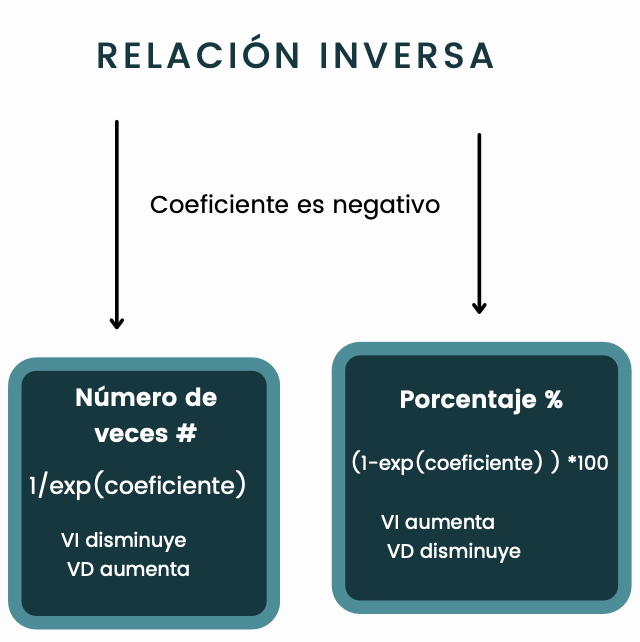
\includegraphics[width=0.3\linewidth]{coef_negativo} \end{center}

{[}Cuando calculcamos el exponencial de los coeficientes, obtenemos el
odds ratio (\# de veces de que ocurra){]}.Sin embargo, como el
coeficiente es negativo esa exponencial debe dividir al 1 (1/exp(log)).

\begin{Shaded}
\begin{Highlighting}[]
\DecValTok{1}\SpecialCharTok{/}\FunctionTok{exp}\NormalTok{(}\FunctionTok{coef}\NormalTok{(modelo1)) }
\end{Highlighting}
\end{Shaded}

\begin{verbatim}
## (Intercept)        P1_4 
##  0.07912577  1.47119355
\end{verbatim}

Siempre que la relación es inversa, la interpretación es cuando la VI
disminuye, la VD aumenta en xx veces. En este caso, 1.47 veces.

Tenemos dos maneras de poner analizar este resultado Recordemos que la
VI era si el o la docente vive con personas de la tercera edad.

\begin{itemize}
\item
  Si el o la docente vive con personas de la tercera edad, el odds de
  que quiera retornar a clases presenciales disminuye en 1.47
\item
  Otra manera analizarlo como una probablilidad, para ello es necesario
  realizar el siguiente cálculo (\textbf{1- exp(coef))*100}
\end{itemize}

Recuerda que el coeficiente de la VI es \emph{-0.3860} es el

\begin{Shaded}
\begin{Highlighting}[]
\NormalTok{(}\DecValTok{1}\SpecialCharTok{{-}}\FunctionTok{exp}\NormalTok{(}\SpecialCharTok{{-}}\FloatTok{0.3860}\NormalTok{))}\SpecialCharTok{*}\DecValTok{100}
\end{Highlighting}
\end{Shaded}

\begin{verbatim}
## [1] 32.02295
\end{verbatim}

En este caso podemos interpretar los resultados como ``si el docente
vive con una persona de la tercera edad, la probabilidad de que quiera
retornar a clases presenciales DISMINUYE en un 32.03\%.

\hypertarget{modelo-2}{%
\section{MODELO 2}\label{modelo-2}}

\hypertarget{realicemos-un-segundo-modelo}{%
\paragraph{REALICEMOS UN SEGUNDO
MODELO}\label{realicemos-un-segundo-modelo}}

Agreguemos más variables:

\begin{itemize}
\item
  vive con personas de la tercera edad (P1\_4)
\item
  ¿sufrió o sufre cancer? (P1\_11\_H)
\item
  ¿sufrió o sufre depresion? (P1\_11\_G)
\end{itemize}

Queremos saber si estas variables influyen en la probabilidad de que el
docente quiera retornar o no a clases presenciales

\begin{Shaded}
\begin{Highlighting}[]
\NormalTok{modelo2 }\OtherTok{=} \FunctionTok{glm}\NormalTok{(retorno }\SpecialCharTok{\textasciitilde{}}\NormalTok{ P1\_4}\SpecialCharTok{+}\NormalTok{P1\_11\_H}\SpecialCharTok{+}\NormalTok{P1\_11\_G, }\AttributeTok{family =}\NormalTok{ binomial,}\AttributeTok{data =}\NormalTok{ data)}
\FunctionTok{summary}\NormalTok{(modelo2)}
\end{Highlighting}
\end{Shaded}

\begin{verbatim}
## 
## Call:
## glm(formula = retorno ~ P1_4 + P1_11_H + P1_11_G, family = binomial, 
##     data = data)
## 
## Deviance Residuals: 
##     Min       1Q   Median       3Q      Max  
## -2.3089   0.3798   0.3798   0.4565   0.7834  
## 
## Coefficients:
##             Estimate Std. Error z value Pr(>|z|)    
## (Intercept)  2.59328    0.03944  65.760  < 2e-16 ***
## P1_4        -0.38429    0.05328  -7.213 5.46e-13 ***
## P1_11_H     -0.92276    0.21281  -4.336 1.45e-05 ***
## P1_11_G     -0.26229    0.06741  -3.891 9.99e-05 ***
## ---
## Signif. codes:  0 '***' 0.001 '**' 0.01 '*' 0.05 '.' 0.1 ' ' 1
## 
## (Dispersion parameter for binomial family taken to be 1)
## 
##     Null deviance: 10576  on 18039  degrees of freedom
## Residual deviance: 10493  on 18036  degrees of freedom
##   (10176 observations deleted due to missingness)
## AIC: 10501
## 
## Number of Fisher Scoring iterations: 5
\end{verbatim}

\begin{Shaded}
\begin{Highlighting}[]
\FunctionTok{coef}\NormalTok{(modelo2)}
\end{Highlighting}
\end{Shaded}

\begin{verbatim}
## (Intercept)        P1_4     P1_11_H     P1_11_G 
##   2.5932761  -0.3842897  -0.9227575  -0.2622864
\end{verbatim}

\hypertarget{ojo-los-tres-coeficientes-son-negativos.-calculemos-el-exponencial}{%
\subsubsection{Ojo, los tres coeficientes son negativos. Calculemos el
exponencial}\label{ojo-los-tres-coeficientes-son-negativos.-calculemos-el-exponencial}}

Para calcular el odds ratio.

\begin{Shaded}
\begin{Highlighting}[]
\FunctionTok{exp}\NormalTok{(}\FunctionTok{coef}\NormalTok{(modelo2)) }
\end{Highlighting}
\end{Shaded}

\begin{verbatim}
## (Intercept)        P1_4     P1_11_H     P1_11_G 
##  13.3735135   0.6809341   0.3974216   0.7692907
\end{verbatim}

Nuevamente, el odds ratio es menor que 1.

Como son menores que 1 entonces lo restamos y explicamos los resultados
en base a la disminución de veces.

\begin{Shaded}
\begin{Highlighting}[]
\DecValTok{1}\SpecialCharTok{/}\NormalTok{(}\FunctionTok{exp}\NormalTok{(}\SpecialCharTok{{-}}\FloatTok{0.38429}\NormalTok{))}
\end{Highlighting}
\end{Shaded}

\begin{verbatim}
## [1] 1.468571
\end{verbatim}

\begin{Shaded}
\begin{Highlighting}[]
\DecValTok{1}\SpecialCharTok{/}\NormalTok{(}\FunctionTok{exp}\NormalTok{(}\SpecialCharTok{{-}}\FloatTok{0.92276}\NormalTok{))}
\end{Highlighting}
\end{Shaded}

\begin{verbatim}
## [1] 2.516226
\end{verbatim}

\begin{Shaded}
\begin{Highlighting}[]
\DecValTok{1}\SpecialCharTok{/}\NormalTok{(}\FunctionTok{exp}\NormalTok{(}\SpecialCharTok{{-}}\FloatTok{0.26229}\NormalTok{))}
\end{Highlighting}
\end{Shaded}

\begin{verbatim}
## [1] 1.299903
\end{verbatim}

Análisis según n° de veces

\begin{itemize}
\item
  Si el docente vive con personas de la tercera edad el
  odds/probabilidad de que quiera retornar a clases presenciales
  disminuye en 1.46 veces
\item
  Si el docente ha tenido o tiene cáncer el odds/probabilidad de que
  quiera retornar a clases presenciales disminuye en 2.51 veces
\item
  Si el docente ha tenido o tiene depresión el odds/probabilidad de que
  quiera retornar a clases presenciales disminuye en 1.29 veces
\end{itemize}

Ahora analicemos las probabilidades:

\begin{Shaded}
\begin{Highlighting}[]
\CommentTok{\#Cuando el odds es menor a 1}
\NormalTok{(}\DecValTok{1}\SpecialCharTok{{-}}\NormalTok{(}\FunctionTok{exp}\NormalTok{(}\SpecialCharTok{{-}}\FloatTok{0.38429}\NormalTok{)))}\SpecialCharTok{*}\DecValTok{100}
\end{Highlighting}
\end{Shaded}

\begin{verbatim}
## [1] 31.90661
\end{verbatim}

\begin{Shaded}
\begin{Highlighting}[]
\NormalTok{(}\DecValTok{1}\SpecialCharTok{{-}}\NormalTok{(}\FunctionTok{exp}\NormalTok{(}\SpecialCharTok{{-}}\FloatTok{0.92276}\NormalTok{)))}\SpecialCharTok{*}\DecValTok{100} 
\end{Highlighting}
\end{Shaded}

\begin{verbatim}
## [1] 60.25794
\end{verbatim}

\begin{Shaded}
\begin{Highlighting}[]
\NormalTok{(}\DecValTok{1}\SpecialCharTok{{-}}\NormalTok{(}\FunctionTok{exp}\NormalTok{(}\SpecialCharTok{{-}}\FloatTok{0.26229}\NormalTok{)))}\SpecialCharTok{*}\DecValTok{100} 
\end{Highlighting}
\end{Shaded}

\begin{verbatim}
## [1] 23.07121
\end{verbatim}

\begin{itemize}
\item
  Si el docente vive con personas de la tercera edad, la probabilidad de
  que quiera retornar a clases presenciales disminuye en 31\%
\item
  Si el docente ha tenido o tiene cáncer la probabilidad de que quiera
  retornar a clases presenciales disminuye en 60\%
\item
  Si el docente ha tenido o tiene depresión la probabilidad de que
  quiera retornar a clases presenciales disminuye en 23\%
\end{itemize}

\hypertarget{si-queremos-calcular-datos-determinados}{%
\paragraph{Si queremos calcular datos
determinados}\label{si-queremos-calcular-datos-determinados}}

Ejemplo 1: Si el docente no vive con personas de la tercera edad, tiene
cancer y tiene depresión

\begin{Shaded}
\begin{Highlighting}[]
\NormalTok{log.odds1 }\OtherTok{=} \FunctionTok{predict}\NormalTok{(modelo2, }\FunctionTok{data.frame}\NormalTok{(}\AttributeTok{P1\_4 =} \DecValTok{0}\NormalTok{, }\AttributeTok{P1\_11\_H =} \DecValTok{1}\NormalTok{, }\AttributeTok{P1\_11\_G =} \DecValTok{1}\NormalTok{))}
\NormalTok{log.odds1}
\end{Highlighting}
\end{Shaded}

\begin{verbatim}
##        1 
## 1.408232
\end{verbatim}

\begin{Shaded}
\begin{Highlighting}[]
\FunctionTok{exp}\NormalTok{(log.odds1)}\SpecialCharTok{/}\NormalTok{(}\DecValTok{1}\SpecialCharTok{+}\FunctionTok{exp}\NormalTok{(log.odds1))}
\end{Highlighting}
\end{Shaded}

\begin{verbatim}
##        1 
## 0.803487
\end{verbatim}

La probabilidad de que quiera retornara a clases presenciales es de 0.80

Ejemplo 2: Si el docente no vive con personas de la tercera edad, no
tiene cancer y tiene depresión

\begin{Shaded}
\begin{Highlighting}[]
\NormalTok{log.odds1 }\OtherTok{=} \FunctionTok{predict}\NormalTok{(modelo2, }\FunctionTok{data.frame}\NormalTok{(}\AttributeTok{P1\_4 =} \DecValTok{0}\NormalTok{, }\AttributeTok{P1\_11\_H =} \DecValTok{0}\NormalTok{, }\AttributeTok{P1\_11\_G =} \DecValTok{1}\NormalTok{))}
\FunctionTok{exp}\NormalTok{(log.odds1)}\SpecialCharTok{/}\NormalTok{(}\DecValTok{1}\SpecialCharTok{+}\FunctionTok{exp}\NormalTok{(log.odds1)) }\CommentTok{\#lo pasamos a probabilidades}
\end{Highlighting}
\end{Shaded}

\begin{verbatim}
##         1 
## 0.9114113
\end{verbatim}

La probabilidad de que quiera retornara a clases presenciales es de 0.91

\hypertarget{ayuda-divina}{%
\subsection{🙌 Ayuda divina 🙌}\label{ayuda-divina}}

Les proponemos esta función (Agradezcanle a su profesor) que facilita la
interpretación de los resultados. La función se llama Divine.Help, para
poder usarla solo necesitas indicar como argumento al nombre de tu
modelo: Divine.Help(modelo). Recuerda que esta función solo podrá
ejecutarse si previamente has ejecutado el código que crea la función.

\begin{Shaded}
\begin{Highlighting}[]
\NormalTok{Divine.Help }\OtherTok{\textless{}{-}} \ControlFlowTok{function}\NormalTok{(model) \{}
   \CommentTok{\# Extraer los coeficientes del modelo}
\NormalTok{  coeficients }\OtherTok{\textless{}{-}} \FunctionTok{coef}\NormalTok{(model)[}\SpecialCharTok{{-}}\DecValTok{1}\NormalTok{] }\CommentTok{\# Excluye el intercepto}
   \CommentTok{\# Inicializar un vector para almacenar los efectos}
\NormalTok{  effects }\OtherTok{\textless{}{-}} \FunctionTok{numeric}\NormalTok{(}\FunctionTok{length}\NormalTok{(coeficients))}
  
  \ControlFlowTok{for}\NormalTok{ (i }\ControlFlowTok{in} \DecValTok{1}\SpecialCharTok{:}\FunctionTok{length}\NormalTok{(coeficients)) \{}
    \ControlFlowTok{if}\NormalTok{ (coeficients[i] }\SpecialCharTok{\textless{}} \DecValTok{1}\NormalTok{) \{}
\NormalTok{      effects[i] }\OtherTok{\textless{}{-}} \FunctionTok{round}\NormalTok{(}\DecValTok{1} \SpecialCharTok{{-}} \FunctionTok{exp}\NormalTok{(coeficients[i]), }\DecValTok{2}\NormalTok{)}
\NormalTok{    \} }\ControlFlowTok{else}\NormalTok{ \{}
\NormalTok{      effects[i] }\OtherTok{\textless{}{-}} \FunctionTok{round}\NormalTok{(}\FunctionTok{exp}\NormalTok{(coeficients[i] }\SpecialCharTok{{-}} \DecValTok{1}\NormalTok{), }\DecValTok{2}\NormalTok{)}
\NormalTok{    \}}
\NormalTok{  \}}
  
   \CommentTok{\# Generar la interpretación en lenguaje natural}
\NormalTok{  interpretation }\OtherTok{\textless{}{-}} \FunctionTok{paste0}\NormalTok{(}\StringTok{"Un aumento de una unidad en la variable "}\NormalTok{, }\FunctionTok{names}\NormalTok{(coeficients),}
                           \StringTok{" está asociado con un cambio de "}\NormalTok{,}
                           \FunctionTok{abs}\NormalTok{(effects)}\SpecialCharTok{*}\DecValTok{100}\NormalTok{, }\StringTok{"\% en la probabilidad de éxito."}\NormalTok{)}
   \CommentTok{\# Devolver los coeficientes, efectos y la interpretación en un dataframe}
\NormalTok{  result }\OtherTok{\textless{}{-}} \FunctionTok{data.frame}\NormalTok{(}\AttributeTok{Coefficient =}\NormalTok{ coeficients,}
                       \AttributeTok{Exp =} \FunctionTok{exp}\NormalTok{(coeficients),}
                       \AttributeTok{Probability =}\NormalTok{ effects,}
                       \AttributeTok{Interpretation =}\NormalTok{ interpretation)}
   \FunctionTok{return}\NormalTok{(result)}
\NormalTok{\}}

\FunctionTok{Divine.Help}\NormalTok{(modelo2)}
\end{Highlighting}
\end{Shaded}

\begin{verbatim}
##         Coefficient       Exp Probability
## P1_4     -0.3842897 0.6809341        0.32
## P1_11_H  -0.9227575 0.3974216        0.60
## P1_11_G  -0.2622864 0.7692907        0.23
##                                                                                                          Interpretation
## P1_4       Un aumento de una unidad en la variable P1_4 está asociado con un cambio de 32% en la probabilidad de éxito.
## P1_11_H Un aumento de una unidad en la variable P1_11_H está asociado con un cambio de 60% en la probabilidad de éxito.
## P1_11_G Un aumento de una unidad en la variable P1_11_G está asociado con un cambio de 23% en la probabilidad de éxito.
\end{verbatim}

\hypertarget{modelo-3}{%
\section{MODELO 3:}\label{modelo-3}}

Nuestras explicativas serán si la persona vive o no con personas de la
tercera edad, tiene o ha tenido ansiedad y la variable edad.

\begin{Shaded}
\begin{Highlighting}[]
\NormalTok{modelo3 }\OtherTok{=} \FunctionTok{glm}\NormalTok{(retorno }\SpecialCharTok{\textasciitilde{}}\NormalTok{ P1\_4}\SpecialCharTok{+}\NormalTok{P1\_11\_F}\SpecialCharTok{+}\NormalTok{P1\_2, }\AttributeTok{family =}\NormalTok{ binomial, }\AttributeTok{data =}\NormalTok{ data)}
\FunctionTok{summary}\NormalTok{(modelo3)}
\end{Highlighting}
\end{Shaded}

\begin{verbatim}
## 
## Call:
## glm(formula = retorno ~ P1_4 + P1_11_F + P1_2, family = binomial, 
##     data = data)
## 
## Deviance Residuals: 
##     Min       1Q   Median       3Q      Max  
## -2.5018   0.3542   0.3997   0.4535   0.6623  
## 
## Coefficients:
##              Estimate Std. Error z value Pr(>|z|)    
## (Intercept)  3.547717   0.137744  25.756  < 2e-16 ***
## P1_4        -0.354417   0.053486  -6.626 3.44e-11 ***
## P1_11_F     -0.437741   0.055822  -7.842 4.44e-15 ***
## P1_2        -0.019287   0.002844  -6.782 1.19e-11 ***
## ---
## Signif. codes:  0 '***' 0.001 '**' 0.01 '*' 0.05 '.' 0.1 ' ' 1
## 
## (Dispersion parameter for binomial family taken to be 1)
## 
##     Null deviance: 10575  on 18034  degrees of freedom
## Residual deviance: 10414  on 18031  degrees of freedom
##   (10181 observations deleted due to missingness)
## AIC: 10422
## 
## Number of Fisher Scoring iterations: 5
\end{verbatim}

Recuerda revisar los signos, para poder identificar el tipo de relación.

\begin{Shaded}
\begin{Highlighting}[]
\FunctionTok{coef}\NormalTok{(modelo3)}
\end{Highlighting}
\end{Shaded}

\begin{verbatim}
## (Intercept)        P1_4     P1_11_F        P1_2 
##  3.54771740 -0.35441669 -0.43774133 -0.01928669
\end{verbatim}

Interpretemos según n° de veces

\begin{Shaded}
\begin{Highlighting}[]
\DecValTok{1}\SpecialCharTok{/}\NormalTok{(}\FunctionTok{exp}\NormalTok{(}\SpecialCharTok{{-}}\FloatTok{0.35441669}\NormalTok{))}
\end{Highlighting}
\end{Shaded}

\begin{verbatim}
## [1] 1.425349
\end{verbatim}

\begin{Shaded}
\begin{Highlighting}[]
\DecValTok{1}\SpecialCharTok{/}\NormalTok{(}\FunctionTok{exp}\NormalTok{(}\SpecialCharTok{{-}}\FloatTok{0.43774133}\NormalTok{))}
\end{Highlighting}
\end{Shaded}

\begin{verbatim}
## [1] 1.549204
\end{verbatim}

\begin{Shaded}
\begin{Highlighting}[]
\DecValTok{1}\SpecialCharTok{/}\NormalTok{(}\FunctionTok{exp}\NormalTok{(}\SpecialCharTok{{-}}\FloatTok{0.01928669}\NormalTok{ ))}
\end{Highlighting}
\end{Shaded}

\begin{verbatim}
## [1] 1.019474
\end{verbatim}

Análisis

\begin{itemize}
\item
  Si el docente vive con personas de la tercera edad el odds de que
  quiera retornar a clases presenciales disminuye en 1.42 veces
\item
  Si el docente ha tenido o tiene ansiedad el odds de que quiera
  retornar a clases presenciales disminuye en 1.54 veces
\item
  Si el docente aumenta en un 1 su edad el odds de que quiera retornar a
  clases presenciales disminuye en 1.01 veces
\end{itemize}

\hypertarget{ahora-en-porcentaje-probabilidad}{%
\paragraph{Ahora en porcentaje
(probabilidad)}\label{ahora-en-porcentaje-probabilidad}}

\begin{Shaded}
\begin{Highlighting}[]
\NormalTok{(}\DecValTok{1}\SpecialCharTok{{-}}\NormalTok{(}\FunctionTok{exp}\NormalTok{(}\SpecialCharTok{{-}}\FloatTok{0.35441669}\NormalTok{))) }\SpecialCharTok{*}\DecValTok{100}
\end{Highlighting}
\end{Shaded}

\begin{verbatim}
## [1] 29.84174
\end{verbatim}

\begin{Shaded}
\begin{Highlighting}[]
\NormalTok{(}\DecValTok{1}\SpecialCharTok{{-}}\NormalTok{(}\FunctionTok{exp}\NormalTok{(}\SpecialCharTok{{-}}\FloatTok{0.43774133}\NormalTok{)))}\SpecialCharTok{*}\DecValTok{100} 
\end{Highlighting}
\end{Shaded}

\begin{verbatim}
## [1] 35.45073
\end{verbatim}

\begin{Shaded}
\begin{Highlighting}[]
\NormalTok{(}\DecValTok{1}\SpecialCharTok{{-}}\NormalTok{(}\FunctionTok{exp}\NormalTok{(}\SpecialCharTok{{-}}\FloatTok{0.01928669}\NormalTok{ )))}\SpecialCharTok{*}\DecValTok{100} 
\end{Highlighting}
\end{Shaded}

\begin{verbatim}
## [1] 1.910189
\end{verbatim}

\begin{itemize}
\item
  Si el docente vive con personas de la tercera edad la probabilidad de
  que quiera retornar a clases presenciales disminuye en 29\%
\item
  Si el docente ha tenido o tiene ansiedad la probabilidad de que quiera
  retornar a clases presenciales disminuye en 35.5\%
\item
  Si el docente aumenta en 1 su edad la probabilidad de que quiera
  retornar a clases presenciales disminuye en 1.9\%
\end{itemize}

Ahora obtengamos la probabilidad según casos

\begin{Shaded}
\begin{Highlighting}[]
\NormalTok{log.odds3 }\OtherTok{=} \FunctionTok{predict}\NormalTok{(modelo3, }\FunctionTok{data.frame}\NormalTok{(}\AttributeTok{P1\_4 =} \DecValTok{0}\NormalTok{, }\AttributeTok{P1\_11\_F =} \DecValTok{1}\NormalTok{, }\AttributeTok{P1\_2 =} \DecValTok{50}\NormalTok{))}
\FunctionTok{exp}\NormalTok{(log.odds3)}\SpecialCharTok{/}\NormalTok{(}\DecValTok{1}\SpecialCharTok{+}\FunctionTok{exp}\NormalTok{(log.odds3))}\CommentTok{\#para pasarlo a probabilidad}
\end{Highlighting}
\end{Shaded}

\begin{verbatim}
##         1 
## 0.8952608
\end{verbatim}

Cuando un o una docente vive con personas de tercera edad, tiene
ansiedad y tenga 50 años, la probabilidad de que quiera retornar a
clases presenciales es de 0.89.

Ahora obtengamos la probabilidad con menor edad.

\begin{Shaded}
\begin{Highlighting}[]
\NormalTok{log.odds3 }\OtherTok{=} \FunctionTok{predict}\NormalTok{(modelo3, }\FunctionTok{data.frame}\NormalTok{(}\AttributeTok{P1\_4 =} \DecValTok{0}\NormalTok{, }\AttributeTok{P1\_11\_F =} \DecValTok{1}\NormalTok{, }\AttributeTok{P1\_2 =} \DecValTok{25}\NormalTok{))}
\FunctionTok{exp}\NormalTok{(log.odds3)}\SpecialCharTok{/}\NormalTok{(}\DecValTok{1}\SpecialCharTok{+}\FunctionTok{exp}\NormalTok{(log.odds3))}
\end{Highlighting}
\end{Shaded}

\begin{verbatim}
##       1 
## 0.93263
\end{verbatim}

Cuando un o una docente vive con personas de tercera edad, tiene
ansiedad y tenga 25 años, la probabilidad de que quiera retornar a
clases presenciales es de 0.93.

\end{document}
